% !TEX TS-program = pdflatex
% !TeX encoding = UTF-8
% !TeX spellcheck = en_GB

%\documentclass[aspectratio=43]{beamer}
% use this instead for 16:9 aspect ratio:
\documentclass[aspectratio=169]{beamer}
% supported acpect ratios  1610  169 149 54 43 (deault) 32
%

\newcommand{\xset}{\mathbb{X}}
\newcommand{\xseti}{\mathbb{X}^{(i)}}
\newcommand{\approxdistri}{q_{\phi}(\textbf{z}|\xseti)}
\newcommand{\approxdistr}{q_{\phi}(\textbf{z}|\xset)}
\newcommand{\truedistr}{p_{\theta}(\textbf{z}|\xseti)}
\newcommand{\elbo}{\mathcal{L}(\theta, \phi; \xseti)}
\newcommand{\xsubset}{\mathbb{X}_k}
\newcommand{\lmopoe}{\mathcal{L}_{MoPoE}(\theta, \phi; \xset)}
\newcommand{\powerset}{\mathcal{P}(\xset)}

\usepackage[english]{babel}
\usepackage[utf8]{inputenc}
\usepackage[T1]{fontenc}

\usepackage{midl_2021/beamerthemeETHbeamer}
%\usetheme{midl_2021/ETHbeamer}

\colorlet{ETHcolor1}{ETHc}
\colorlet{ETHcolor2}{ETHi}

\usepackage{tikz}
\usepackage{graphicx}
\usepackage{graphviz}
\usepackage{amsfonts}
\usepackage{mathtools}
\usepackage{tikz}
%\usepackage{authblk}
\usetikzlibrary{shapes,snakes}

%BIBLIOGRAPHY
% see https://mirror.foobar.to/CTAN/macros/latex/contrib/biblatex/doc/biblatex.pdf for available styles
\usepackage[backend=bibtex,style=authoryear,natbib=true]{biblatex}
\addbibresource{bib.bib}

\author{Hendrik Klug, Thomas M. Sutter, Julia E. Vogt}
%\author[shortname]{First Author \textsuperscript{1} \and Second Author \inst{1, 2} \and Fourth Author \inst{2,3}}
%\institute[shortinst]{\textsuperscript{1} ITMO University \and \inst{2} University of Whatever \and \inst{3} Whatever Institute}


\title{Multimodal Generative Learning on the MIMIC-CXR Database}

\date{}

% uncomment if you do not want to use a department logo
%\deplogofalse


\begin{document}

    \titleframe

    \begin{frame}
        In this work, we applied a method for \textbf{self-supervised}, \textbf{multimodal} and \textbf{generative} training proposed by Sutter et al. \footcite{thomas_multimodal} on medical data from the MIMIC-CXR Database \footcite{johnson2019mimic}.
    \end{frame}


    \begin{frame}{Self-supervised, multimodal, generative learning}
        \resizebox{\textwidth}{!}{%
            \begin{tikzpicture}[modalities/.style={rectangle, draw=green!60, fill=green!5, very thick, minimum size=5mm},model/.style={rectangle, draw=red!60, fill=red!5, very thick, minimum size=20mm},lr/.style={ellipse, draw=blue!60, fill=blue!5, very thick, minimum height=5mm,  minimum width=10mm}]
                \node[modalities] (input_text) {Text};
                \node[modalities, below of=input_text] (input_F) {F-Img};
                \node[modalities, below of=input_F] (input_L) {L-Img};
                \node[model, right of=input_F, xshift=2cm] (encoder) {Encoder};
                \node[lr, right of=encoder, xshift=3cm, align=center] (lr) {Latent\\ Representation  \footnote{Assumed to be Gaussian distributed}};
                \node[model, right of=lr, xshift=3cm] (decoder) {Decoder};
                \node[modalities, right of=decoder, xshift=2cm] (out_F) {F-Img};
                \node[modalities, below of=out_F] (out_L) {L-Img};
                \node[modalities, above of=out_F] (out_text) {Text};
                \draw[->] (input_text) -- (encoder);
                \draw[->] (input_F) -- (encoder);
                \draw[->] (input_L) -- (encoder);
                \draw[->] (encoder) -- (lr);
                \draw[->] (lr) -- (decoder);
                \draw[->] (decoder) -- (out_F);
                \draw[->] (decoder) -- (out_text);
                \draw[->] (decoder) -- (out_L);
            \end{tikzpicture}}
    \end{frame}

    \begin{frame}{Multimodal, Unsupervised Generative Learning On Medical Data}
        \large{The advantages:}
        \pause
        \begin{itemize}
            \item No need for labeled data
        \end{itemize}
    \end{frame}

    \begin{frame}{No need for labeled data}
        \begin{itemize}
            \item Model is trained to reconstruct the input image $\rightarrow$ no need for labels
            \item Big advantage over other methods:
            \begin{itemize}
                \item In the medical domain, labeling data requires manual expert input
                \item Labeled medical data is only a small subset of all the medical data available
            \end{itemize}
        \end{itemize}
    \end{frame}



    \begin{frame}{Multimodal, Unsupervised Generative Learning On Medical Data}
        \large{The advantages:}
        \begin{itemize}
            \item No need for labeled data
            \item Can extract features and generate from multiple modalities that exist in the medical domain:
            \pause
            \begin{itemize}
                \item Radiographs from multiple angles or different imaging technologies
                \item Text reports
                \item Electronic health records
            \end{itemize}
            \pause
            \item Can \textbf{generate} \textit{coherent} samples
            \pause
            \item Learned latent representation can be used for \textbf{classification}
            \begin{itemize}
                \item Semantically close samples will be grouped together in the learned latent representation.
            \end{itemize}
        \end{itemize}
    \end{frame}


    \begin{frame}{Example Applications}
        \begin{itemize}
            \pause
            \item Relieve doctors from the tedious task of writing summary text report by generating it.
            \pause
            \item Generating a lateral view image from a frontal view one or vice versa.
            \pause
            \begin{itemize}
                \item Reduce cost for each patient
                \item Reduce radiation in the case of X-ray imaging
            \end{itemize}
            \pause
            \item The classification ability could support the judgement of a clinician.
        \end{itemize}

    \end{frame}


    \section{Background}

    \subsection{The MoPoE-VAE (\cite{thomas_gener-ELBO})}
    \begin{frame}{The Mixture-of-Products-of-Experts-VAE (MoPoE)}
        The multimodal aspect has many advantages, but \textbf{combining the learned distributions for each modality into a joint latent distribution is still an open problem}.
    \end{frame}

    \begin{frame}{The Mixture-of-Products-of-Experts-VAE (MoPoE)}
        Here we used a method from \cite{thomas_gener-ELBO}, which is a combination of:
        \begin{itemize}
            \item The Product-of-Experts (PoE) from \cite{wu2018multimodal}
            \item The Mixture-of-Experts (MoE) from \cite{shi2019variational}
        \end{itemize}
    \end{frame}


    \section{Methods}

    \subsection{The MIMIC-CXR Database}

    \begin{frame}{The MIMIC-CXR Database}
        \pause
        \begin{itemize}
            \item Published in \cite{johnson2019mimic}
            \item Consists of:
            \begin{itemize}
                \item Chest radiographs
                \item Text reports
            \end{itemize}

        \end{itemize}
    \end{frame}

    \begin{frame}
        \begin{figure}
            \centering
            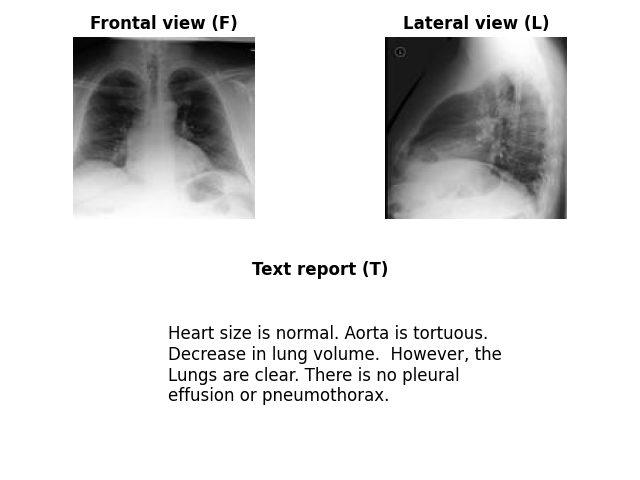
\includegraphics[width=0.6\textwidth]{data/rand_dataset_sample.png}
        \end{figure}

    \end{frame}

    \begin{frame}{The Labels}
        \pause
        \begin{itemize}
            \item Because the labels are highly unbalanced, we created a binary label "Finding".
            \begin{itemize}
                \item If sample presents any pathology $\rightarrow$ finding = True, else False
            \end{itemize}
            \item This results in 14529 samples that are annotated with the "Finding" label in the training set and 47218 samples that are not.
        \end{itemize}
    \end{frame}

%    \begin{frame}{The text processing}
%
%        \small{
%            "Heart size is normal." $\rightarrow [0,1,2,3] \rightarrow$ Model $\rightarrow
%            \begin{bsmallmatrix}
%                1 & 0 & 0 & 0\\
%                0 & 1 & 0 & 0\\
%                0 & 0 & 1 & 0\\
%                0 & 0 & 0 & 1\\
%            \end{bsmallmatrix}$
%            $\rightarrow [0,1,2,3] \rightarrow$ "Heart size is normal."}\\
%        \vspace{\baselineskip}
%        \pause
%        \begin{itemize}
%            \item Every word that occurs at least 3 times in all the text reports is mapped to an index.
%            \pause
%            \item Using this mapping each sentence is encoded into a sequence of indices.
%            \pause
%            \item The output of the decoder is in a one-hot-encoded format.
%        \end{itemize}
%    \end{frame}
%
%    \subsection{The model architecture}
%    \begin{frame}{The model}
%        \begin{itemize}
%            \item The MoPoE-VAE has an independent encoder and decoder for each modality (F, L and T).
%            \item In this work we used a ResNet \footcite{he2016deep} type architecture with 6 residual blocks for all encoders and decoders.
%        \end{itemize}
%
%    \end{frame}


    \section{Results}

    \begin{frame}{Mean AP for the MoPoE}
        \begin{table}
            \centering
            \begin{tabular}{lcccccccc}
                MODEL & F     & L     & T     & L,F   & F,T   & L,T   & L,F,T          \\
                \hline
                MoPoE & 0.467 & 0.460 & 0.473 & 0.476 & 0.493 & 0.475 & \textbf{0.494} \\
                Random & \multicolumn{6}{c}{0.235}
            \end{tabular}
            \caption{\textbf{Classification results of the linear classifiers trained on the learned latent representation using the binary label "Finding". The mean average precision over the test set
            is reported for each subset (F: frontal image, L: lateral image, T: text report).}}
        \end{table}
    \end{frame}


    \begin{frame}{Conditionally generated samples with L and T modalities as conditioner.}

        \begin{figure}
%            \centering
            \vspace{-0.1\textheight}
            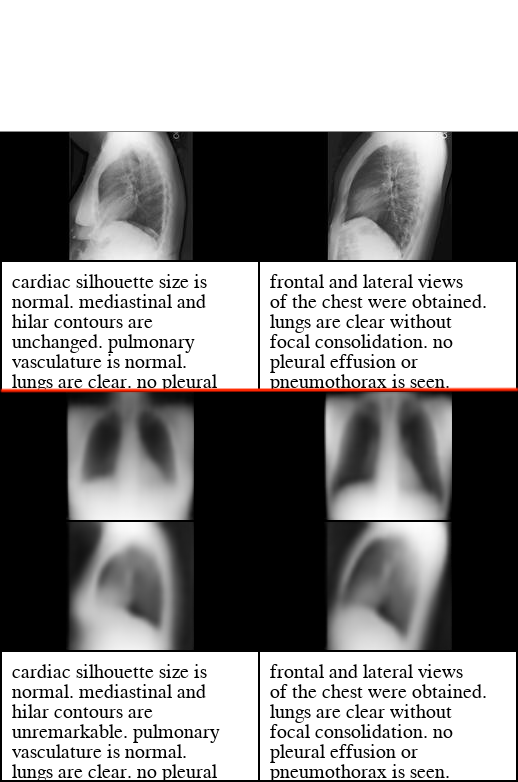
\includegraphics[width=0.6\textwidth, height = 0.75\textheight, keepaspectratio]{data/cond_gen/Lateral_text_small_edited.png}

        \end{figure}
    \end{frame}

    \begin{frame}{Adding the F modality as conditioner}
        \begin{figure}
            \centering
            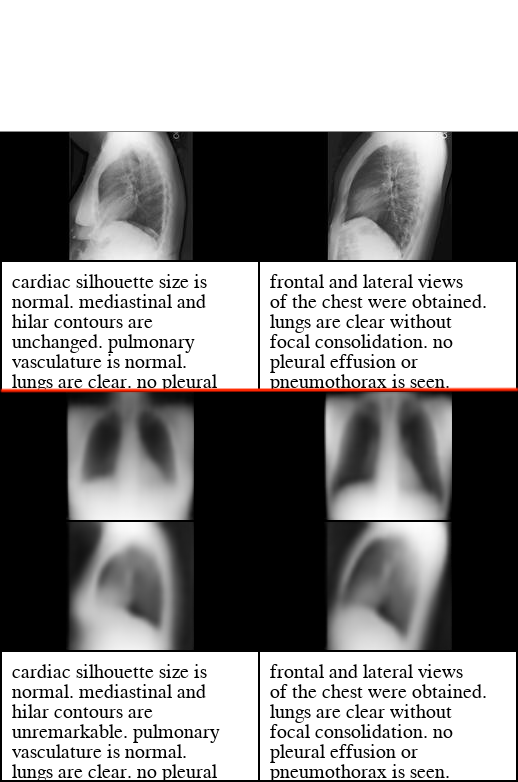
\includegraphics[width=0.6\textwidth, height = 0.75\textheight, keepaspectratio]{data/cond_gen/Lateral_text_small_edited.png}
            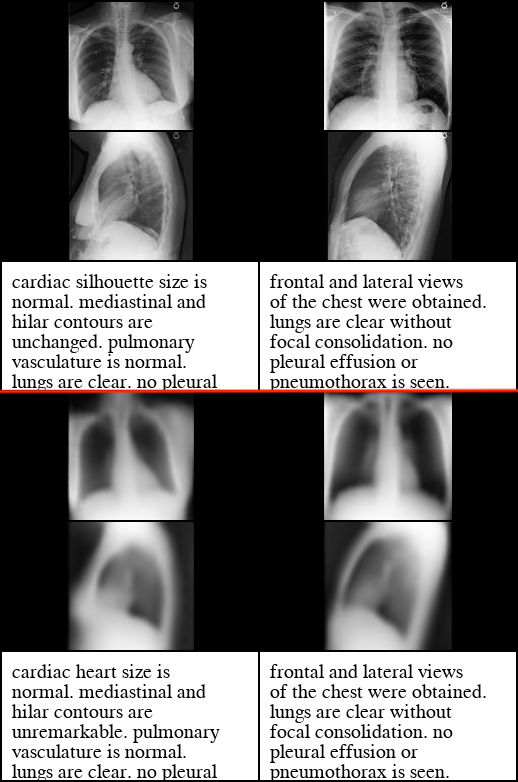
\includegraphics[width=0.6\textwidth, height = 0.75\textheight, keepaspectratio]{data/cond_gen/Lateral_PA_text_small_edited.png}
        \end{figure}
    \end{frame}


    \section{Conclusion}
    \begin{frame}{Conclusion}
        We showed that:
        \begin{itemize}
            \item The MoPoE method provides promising results when applied to medical data for:
            \begin{itemize}
                \item Classification
                \item Generation
            \end{itemize}
            \item However, we also highlighted some problems that can still be addressed to improve the performance.
        \end{itemize}
    \end{frame}

    \begin{frame}{Future Work}
        \begin{itemize}
            \item Finding better architecture for the decoder and encoder parts.
            \item Finding a better prior than the Gaussian distribution. \footcite{zhao2017towards}
            \item Trying state-of-the-art method such as
            \begin{itemize}
                \item Vector Quantised-Variational AutoEncoder \footcite{oord2018neural}
                \item Deep Hierarchical Variational AutoEncoder \footcite{vahdat2021nvae}
            \end{itemize}

        \end{itemize}

    \end{frame}

    \printbibliography


\end{document}
